\subsection{Explainability}

A final interesting point in comparing different SL-techniques is their explainability. Figure \ref{fig:7_explain_tradeoff} shows a potentially existing trade-off, where more complex and therefore less explainable techniques have a better quality of prediction.

\begin{figure}[H]
  \centering
  \begin{subfigure}{0.8\textwidth}
    \centering
    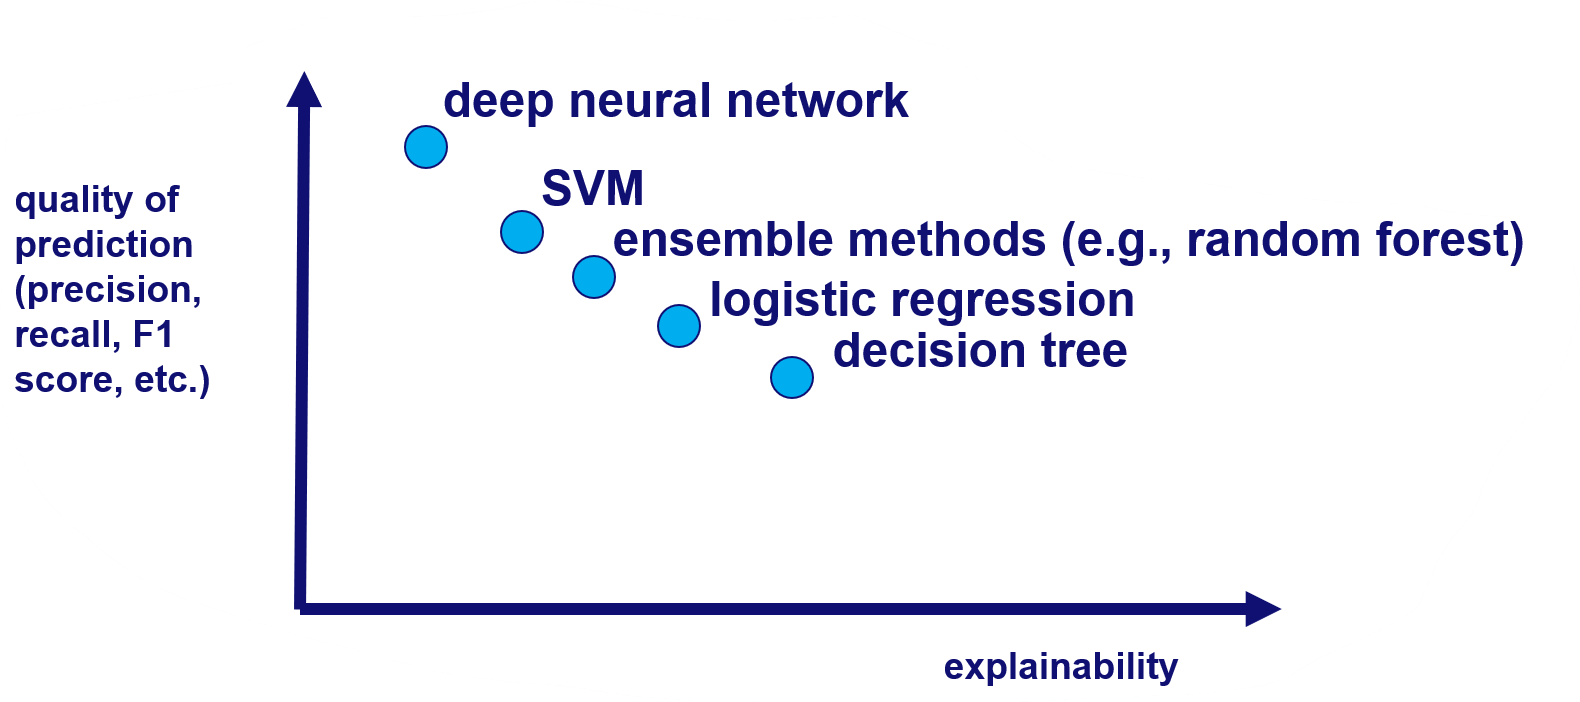
\includegraphics[width=\textwidth]{assets/sl/explain__tradeoff.png}
    \begin{note}
      Positions are just indications, true positions depend on many factors (data set, parameters, ...)

      DNN can perform very poorly on small data sets
    \end{note}
  \end{subfigure}

  \caption{Quality of prediction vs. explainability}
  \label{fig:7_explain_tradeoff}
\end{figure}

As one can see: especially DNNs are not explainable. Whether the system derives:
\begin{itemize}
  \item Guilty because of $X\& Y\& Z$, or
  \item If $X \& Y \& Z$, then guilty
\end{itemize}
Can't be told so far (so not really good judges $\rightarrow$ true reasoning not tellable).

Similar example: using an NN as a doctor can lead to it telling you that you have an $80\%$ chance of dying, but not why IF it is poorly developed and applied.